\chapter{Description of mini project concept}

Seeing how our semester project was a demining robot, it only seemed fitting for us to make a mining-robot for this project - this robot does however not lay landmines, it mines minerals.\\
\\
The basic idea was to make something similar to a computer game, so we took the tile based movement known from especially turn based role playing games and mixed in the time\footnote{Turn 90 \textdegree = 30 sec. Turn 180 \textdegree = 50 sec. Move one tile forward = 45 sec. Move two tiles forward = 80 sec. Move one tile backwards = 55 sec. Mine one unit of mineral = 60 sec. Check if cart is full = 10 sec. Unload cart = 70 sec.} aspect of real-time strategy games. The result was a mining robot which the user could command to perform simple tasks in a fictive mine.

\begin{figure}[!ht]
  \centering
  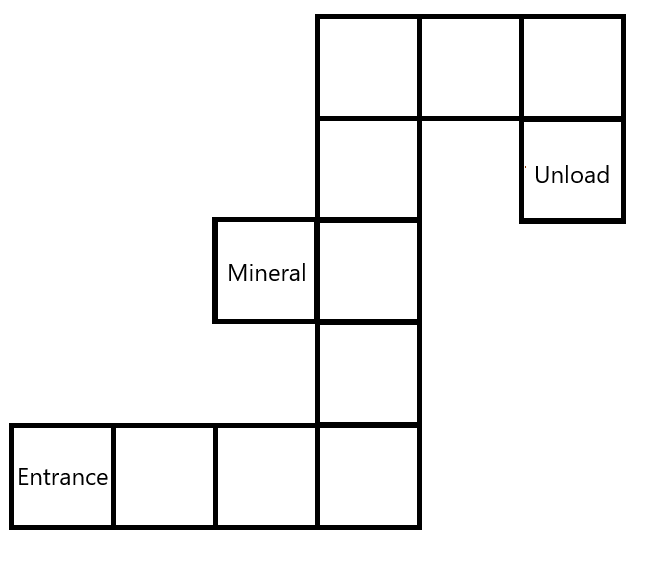
\includegraphics[width=6cm]{RPro-Mini-Project-B332b/00 - Images/mineMap.png}
  \caption{Map of the fictive mine}
\end{figure}

The robot wills perform the tasks as they are coded and output progress and results to a subscriber node. This can be compared to the text display often found in RPGs, where the player can see a text output of what is happening on screen.\\
\\
This is obviously only a small snippet, but it could be seen as a demonstration of how a single element of a larger computer game would behave and communicate as well as be manipulated by the user.\\
\\
